\documentclass[tikz,border=10pt]{standalone}
\usetikzlibrary{arrows.meta, positioning, shapes.geometric}

\begin{document}
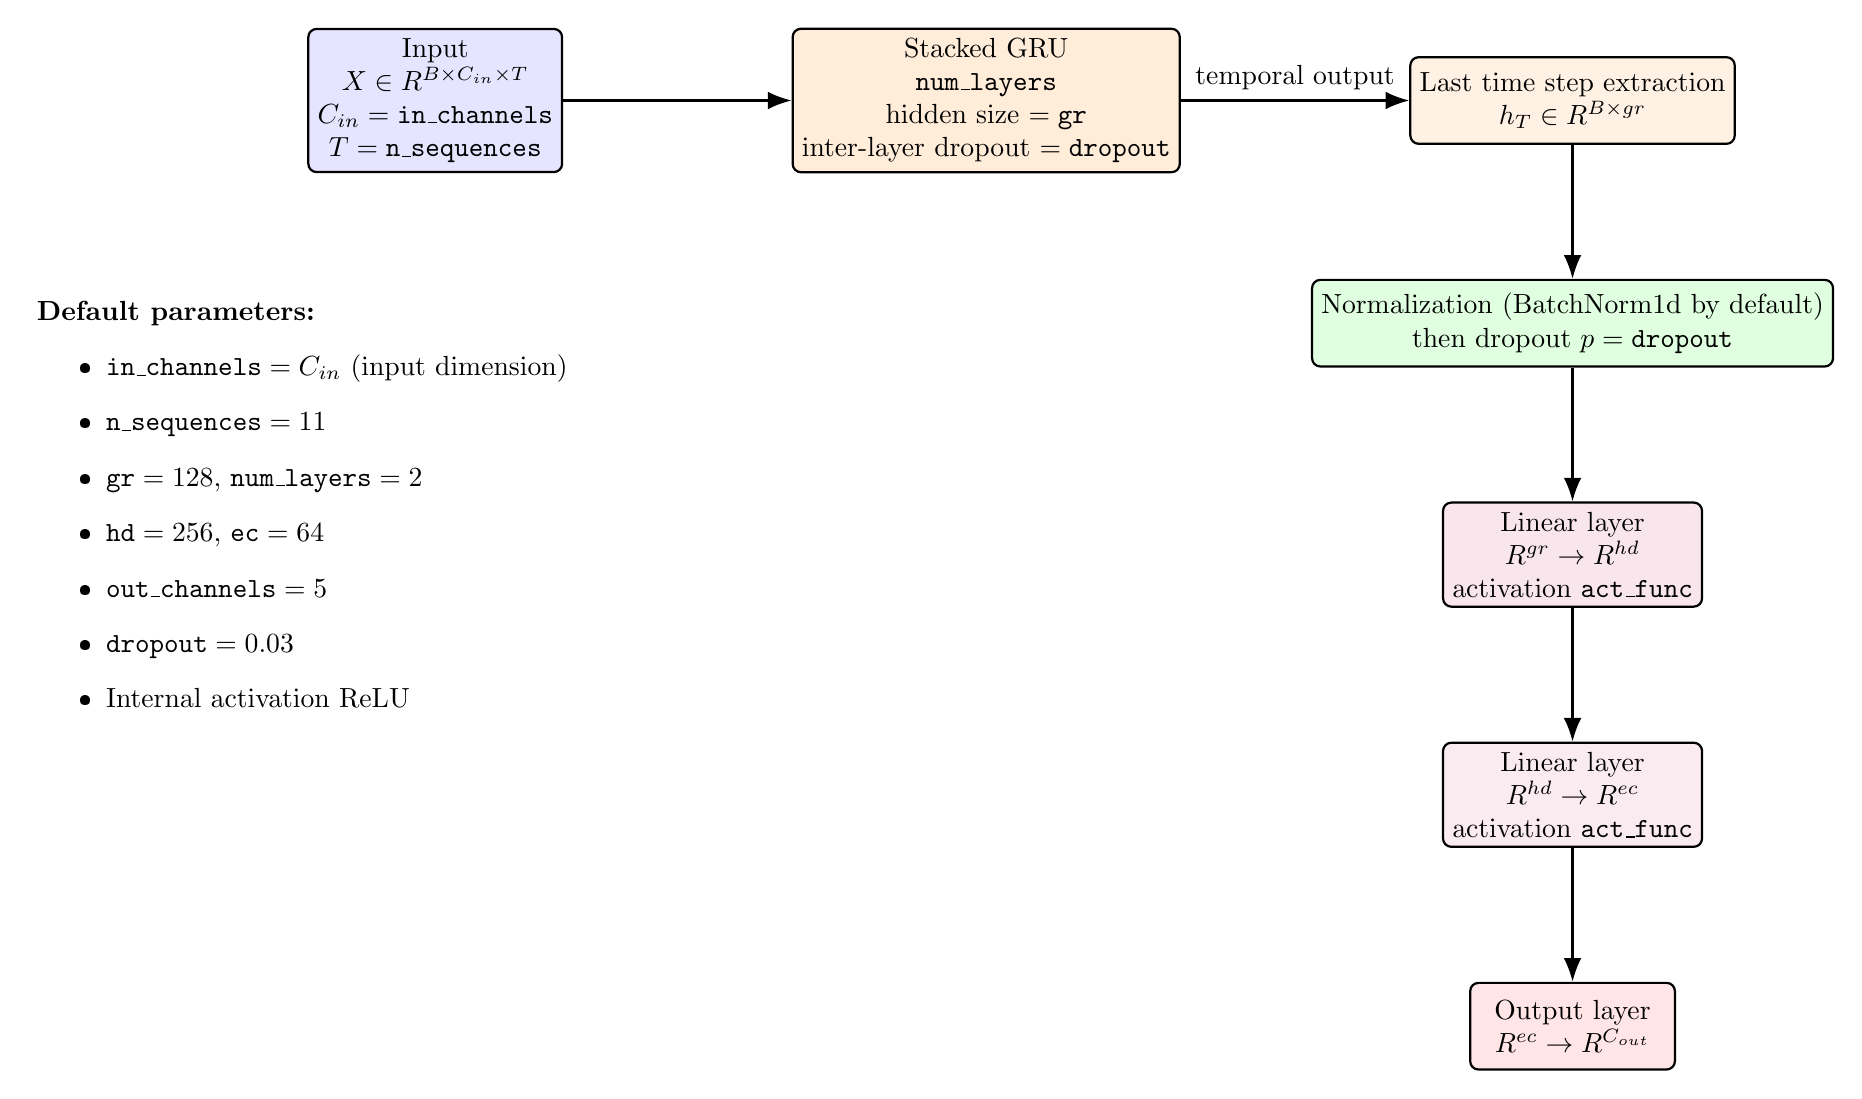
\begin{tikzpicture}[
    block/.style={draw, thick, minimum width=2.6cm, minimum height=1.1cm, align=center, rounded corners=3pt},
    arrow/.style={-{Latex[length=3mm]}, thick}
]
    % Input sequence information
    \node[block, fill=blue!10] (input) {Input\\$X \in \mathbb{R}^{B \times C_{in} \times T}$\\
        $C_{in} = \texttt{in\_channels}$\\
        $T = \texttt{n\_sequences}$};

    % GRU block
    \node[block, right=2.9cm of input, fill=orange!15] (gru) {Stacked GRU\\
        $\texttt{num\_layers}$\\
        hidden size $= \texttt{gr}$\\
        inter-layer dropout $= \texttt{dropout}$};

    \draw[arrow] (input) -- (gru);

    % Last timestep extraction
    \node[block, right=2.9cm of gru, fill=orange!10] (last) {Last time step extraction\\
        $h_T \in \mathbb{R}^{B \times gr}$};

    \draw[arrow] (gru) -- node[above]{temporal output} (last);

    % Normalization & dropout
    \node[block, below=1.7cm of last, fill=green!12] (norm) {Normalization (BatchNorm1d by default)\\then dropout $p=\texttt{dropout}$};

    \draw[arrow] (last) -- (norm);

    % Linear layers and activations
    \node[block, below=1.7cm of norm, fill=purple!10] (linear1) {Linear layer\\$\mathbb{R}^{gr} \rightarrow \mathbb{R}^{hd}$\\
        activation $\texttt{act\_func}$};

    \draw[arrow] (norm) -- (linear1);

    \node[block, below=1.7cm of linear1, fill=purple!8] (linear2) {Linear layer\\$\mathbb{R}^{hd} \rightarrow \mathbb{R}^{ec}$\\
        activation $\texttt{act\_func}$};

    \draw[arrow] (linear1) -- (linear2);

    \node[block, below=1.7cm of linear2, fill=red!10] (output) {Output layer\\$\mathbb{R}^{ec} \rightarrow \mathbb{R}^{C_{out}}$};

    \draw[arrow] (linear2) -- (output);

    % Legends for parameters
    \node[below=1.5cm of input, align=left] (legend) {
        \begin{minipage}{10cm}
            \textbf{Default parameters:}
            \begin{itemize}
                \item $\texttt{in\_channels} = C_{in}$ (input dimension)
                \item $\texttt{n\_sequences} = 11$
                \item $\texttt{gr} = 128$, $\texttt{num\_layers} = 2$
                \item $\texttt{hd} = 256$, $\texttt{ec} = 64$
                \item $\texttt{out\_channels} = 5$
                \item $\texttt{dropout} = 0.03$
                \item Internal activation ReLU
            \end{itemize}
        \end{minipage}
    };

\end{tikzpicture}
\end{document}
